\documentclass{article}
\usepackage{amsmath, sfmath, multicol, tkz-euclide, array, enumerate, tcolorbox, tabularray}
\renewcommand{\familydefault}{\sfdefault}
\setlength{\parindent}{0cm}
\pagestyle{empty}
\usepackage[left=1in, top=0.5in, right=1in, bottom=0.5in]{geometry}
% \usetikzlibrary{arrows}
\tikzset{>=stealth}
\tcbset{colback=white}

\newcounter{example}[section]
\newenvironment{example}[1][]{\refstepcounter{example}\par\medskip
   {\color{red}\textbf{Example~\theexample. #1}}}{\medskip}

\begin{document}

\section*{Parallel Lines}

\begin{tcolorbox}[colframe=orange!70!white, coltitle=black, title=\textbf{Today I Can}]
\begin{enumerate}
    \item Use properties of parallel lines to find angle measures.
\end{enumerate}
\end{tcolorbox}

\begin{tcolorbox}[colframe=black!20!white, opacitybacktitle=0.1, coltitle=black, title=\textbf{Parallel Lines}]
Two coplanar lines are parallel if they do not intersect. \newline 

\begin{minipage}{0.5\textwidth}
\begin{itemize}
    \item $\overline{AB} \parallel \overline{CD}$
\end{itemize}
\end{minipage}
\begin{minipage}{0.4\textwidth}
\begin{tikzpicture}
\tkzDefPoints{0/0/O, -1.5/0/A, 1.5/0/B}
\tkzDrawSegments[<->, add = 0.5 and 0.5](A,B)
\tkzDefShiftPoint[O](-1,-1){O1}
\tkzDefShiftPoint[O1](180:1.5){C}
\tkzDefShiftPoint[O1](0:1.5){D}
\tkzDrawSegments[<->, add = 0.5 and 0.5](C,D)
\tkzDrawPoints(A,B,C,D)
\tkzLabelPoints(A,B,C,D)
% \tkzDrawSegment[<->, add = 0.5 and 0.5](O,O1)
\end{tikzpicture}
\end{minipage}
\end{tcolorbox}

\begin{tcolorbox}[colframe=black!20!white, opacitybacktitle=0.1, coltitle=black, title=\textbf{Transversal Line}]
A line that intersects 2 or more coplanar lines at distinct points. 

\begin{minipage}{0.5\textwidth}
\begin{itemize}
    \item $\ell$ is a transversal line
\end{itemize}
\end{minipage}
\begin{minipage}{0.4\textwidth}
\begin{tikzpicture}
\tkzDefPoints{0/0/O, -1.5/0/A, 1.5/0.25/B}
\tkzDrawSegments[<->, add = 0.5 and 0.5](A,B)
\tkzDefShiftPoint[O](-1,-1){O1}
\tkzDefShiftPoint[O1](180:1.5){C}
\tkzDefShiftPoint[O1](0:1.5){D}
\tkzDrawSegments[<->, add = 0.5 and 0.5](C,D)
% \tkzDrawPoints(A,B,C,D)
% \tkzLabelPoints(A,B,C,D)
\tkzDrawSegment[<->, add = 0.5 and 0.5](O,O1)
\tkzLabelSegment[pos=1.5](O1,O){$\ell$}
\end{tikzpicture}
\end{minipage}
\end{tcolorbox}

\subsection*{Parallel Lines and Transversals} \bigskip 

\begin{center}
\begin{tikzpicture}[decoration={markings,
mark=at position 0.75 with {\arrow[scale=2]{>}};}]
    \tkzDefPoints{0/0/A, -1.75/0/B, 1.75/0/C}
    \tkzDefShiftPoint[A](70:1.5){D}
    \tkzDefShiftPoint[D](0:2){F}
    \tkzDefShiftPoint[D](180:2){E}
    \tkzDrawSegments[add = 0.25 and 0.25, <->, >=stealth](B,C F,E)
    \tkzDrawSegments[add = 0.5 and 0.5, <->, >=stealth](A,D)
    \tkzMarkSegments[mark=>](A,C D,F)
    %\tkzLabelPoints(A,B,C,D,E,F)
    \node at (D) [anchor = south east] {1};
    \node at (65:1.6) [anchor = south west] {2};
    \node at (D) [anchor = north west] {4};
    \node at (75:1.4) [anchor = north east] {3};
    \node at (A) [anchor = south east] {5};
    \node at (25:0.25) [anchor = south west] {6};
    \node at (A) [anchor = north west] {7};
    \node at (200:0.15) [anchor = north east] {8};
\end{tikzpicture}
\end{center}

\subsubsection*{Angle Relationships with Parallel Lines and Transversals}

\setlength{\extrarowheight}{3pt}
\begin{tabular}{|c|c|c|c|c|}
\hline
Corresponding    &
Alternate Interior   &
Alternate Exterior   &
Same-Side Interior   &
Same-Side Exterior   \\[3pt] \hline
\textbullet 1 and 5 &   &   &   &   \\
\textbullet 2 and 6 &
\textbullet 3 and 6 &
\textbullet 2 and 7 &
\textbullet 3 and 5 &
\textbullet 1 and 7 \\
\textbullet 3 and 7 &
\textbullet 4 and 5 &
\textbullet 1 and 8 &
\textbullet 4 and 6 &
\textbullet 2 and 8 \\
\textbullet 4 and 8 &   &   &   &   \\[3pt]  \hline
\end{tabular}
\vspace{0.25in}

\begin{example}
Find the measure of each angle given each pair of parallel lines.

\begin{multicols}{2}
\begin{enumerate}[(a)]
\item \mbox{} \newline\\
\begin{tikzpicture}[decoration={markings,
mark=at position 0.75 with {\arrow[scale=2]{>}};}]
    \tkzDefPoints{0/0/A, -1.5/0/B, 1.5/0/C}
    \tkzDrawSegments[add = 0.25 and 0.25, <->, >=stealth](B,C)
    \tkzDefShiftPoint[A](110:1.5){D}
    \tkzDefShiftPoint[D](0:1.5){E}
    \tkzDefShiftPoint[D](180:0.5){F}
    \tkzDrawSegments[add = 0.75 and 0.75, <->, >=stealth](E,F A,D)
    \tkzMarkSegments[mark=>](A,C D,E)
  % \tkzLabelPoints(A,B,C,D,E,F)
    \tkzLabelAngle[pos=0.5](E,D,A){$70^\circ$}
    \tkzLabelAngle[pos=0.25](C,A,F){?}
\end{tikzpicture}

\item \mbox{} \newline\\
\begin{tikzpicture}[decoration={markings,mark=at position 0.75 with {\arrow[scale=2]{>}};}]
    \tkzDefPoints{0/0/A, -1.5/0/B, 1.5/0/C}
    \tkzDrawSegments[add = 0.25 and 0.25, <->, >=stealth](B,C)
    \tkzDefShiftPoint[A](88:1.5){D}
    \tkzDefShiftPoint[D](0:1.5){E}
    \tkzDefShiftPoint[D](180:0.5){F}
    \tkzDrawSegments[add = 0.75 and 0.75, <->, >=stealth](E,F A,D)
    \tkzMarkSegments[mark=>](A,C D,E)
   %\tkzLabelPoints(A,B,C,D,E,F)
    \tkzLabelAngle[pos=0.5](E,D,A){$92^\circ$}
    \tkzLabelAngle[pos=-0.35](B,A,F){?}
\end{tikzpicture}

\end{enumerate}
\end{multicols}
\end{example}

\newpage

\begin{example}
Find the value of the variable in each.
\begin{multicols}{2}
\begin{enumerate}[(a)]
\item \mbox{} \newline 
\begin{tikzpicture}[decoration={markings,
mark=at position 0.5 with {\arrow[scale=2]{>}};}]
    \tkzDefPoints{0/0/A, -1.5/0/B, 1.5/0/C}
    \tkzDrawSegments[add = 0.25 and 0.25, <->, >=stealth](B,C)
    \tkzDefShiftPoint[A](110:1.5){D}
    \tkzDefShiftPoint[D](0:1.5){E}
    \tkzDefShiftPoint[D](180:0.5){F}
    \tkzDrawSegments[add = 0.75 and 0.75, <->, >=stealth](E,F A,D)
    \tkzMarkSegments[mark = >](A,C D,E)
    \node at (A) [anchor = south east] {$x+76$};
    \node at (F) [anchor = north] {$110^\circ$};
\end{tikzpicture}

\item \mbox{} \newline 
\begin{tikzpicture}[decoration={markings,
mark=at position 0.75 with {\arrow[scale=2]{>}};}]
    \tkzDefPoints{0/0/A, -1.5/0/B, 1.5/0/C}
    \tkzDrawSegments[add = 0.25 and 0.25, <->, >=stealth](B,C)
    \tkzDefShiftPoint[A](100:1.5){D}
    \tkzDefShiftPoint[D](0:1.5){E}
    \tkzDefShiftPoint[D](180:0.5){F}
    \tkzDrawSegments[add = 0.75 and 0.75, <->, >=stealth](E,F A,D)
    \tkzMarkSegments[mark=>](A,C D,E)
   %\tkzLabelPoints(A,B,C,D,E,F)
    \node at (A) [anchor = north east] {$-10+11x$};
    \node at (F) [anchor = north] {$100^\circ$};
\end{tikzpicture}
\end{enumerate}
\end{multicols}
\end{example}

\vfill 

\begin{example}
Find the measure of the angle in bold.

\begin{multicols}{2}
\begin{enumerate}[(a)]
\item \mbox{} \newline
\begin{tikzpicture}[decoration={markings,
mark=at position 0.5 with {\arrow[scale=2]{>}};}]
    \tkzDefPoints{0/0/A, -1.5/0/B, 1.5/0/C}
    \tkzDrawSegments[add = 0.25 and 0.25, <->, >=stealth](B,C)
    \tkzDefShiftPoint[A](120:1.5){D}
    \tkzDefShiftPoint[D](0:1.5){E}
    \tkzDefShiftPoint[D](180:0.5){F}
    \tkzDrawSegments[add = 0.75 and 0.75, <->, >=stealth](E,F A,D)
    \tkzMarkSegments[mark=>](D,E B,A)
   %\tkzLabelPoints(A,B,C,D,E,F)
    \node at (A) [anchor = south west] {$\mathbf{23\textit{x}+5}$};
    \node at (F) [anchor = north] {$24x$};
\end{tikzpicture}

\item \mbox{} \newline
\begin{tikzpicture}[decoration={markings,
mark=at position 0.85 with {\arrow[scale=2]{>}};}]
    \tkzDefPoints{0/0/A, -1.5/0/B, 1.5/0/C}
    \tkzDrawSegments[add = 0.25 and 0.25, <->, >=stealth](B,C)
    \tkzDefShiftPoint[A](75:1.5){D}
    \tkzDefShiftPoint[D](0:1.5){E}
    \tkzDefShiftPoint[D](180:0.5){F}
    \tkzDrawSegments[add = 0.75 and 0.75, <->, >=stealth](E,F A,D)
    \tkzMarkSegments[mark=>](A,C D,E)
   %\tkzLabelPoints(A,B,C,D,E,F)
    \node at (D) [anchor = south west] {$\mathbf{4\textit{\textbf{x}}\textbf{+}4}$};
    \node at (A) [anchor = north east] {$6x-4$};
\end{tikzpicture}
\end{enumerate}
\end{multicols}
\end{example}

\vfill 

\begin{example}
Find the value of the variable in each.

\begin{multicols}{2}
\begin{enumerate}[(a)]
\item \mbox{} \newline
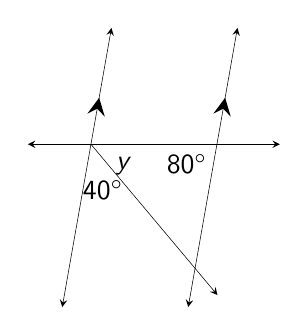
\begin{tikzpicture}[decoration={markings,
mark=at position 0.5 with {\arrow[scale=2]{>}};}, scale=0.8]
    \tkzDefPoints{0/0/A, 2/0/B}
    \tkzDefShiftPoint[A](80:1.5){C}
    \tkzDefShiftPoint[B](80:1.5){D}
    \tkzDrawSegments[add = 0.25 and 1.75, <->, >=stealth](C,A D,B)
    \tkzDrawSegments[add = 0.5 and 0.5, <->, >=stealth](A,B)
    %\tkzLabelPoints(A,B,C,D)
    \tkzMarkSegments[mark=>](A,C B,D)
    \tkzDefShiftPoint[A](-50:2.5){E}
    \tkzDrawSegments[add = 0 and 0.25, ->, >=stealth](A,E)
    \node at (-10:0.25) [anchor = north west] {$y$};
    \node at (-75:0.75) {$40^\circ$};
    \node at (B) [anchor = north east] {$80^\circ$};
\end{tikzpicture}

\item \mbox{} \newline
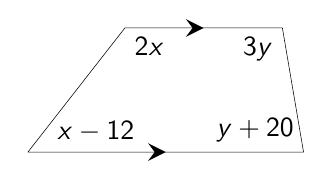
\begin{tikzpicture}[decoration={markings,
mark=at position 0.5 with {\arrow[scale=2]{>}};}]
    \tkzDefPoints{0/0/A, 3.5/0/B}
    \tkzDefShiftPoint[A](52:2){C}
    \tkzDefShiftPoint[C](0:2){D}
    \tkzDrawPolygon(A,B,D,C)
    \tkzMarkSegments[mark=>](A,B C,D)
    \node at (0.25,0) [anchor = south west] {$x-12$};
    \node at (C) [anchor = north west] {$2x$};
    \node at (D) [anchor = north east] {$3y$};
    \node at (B) [anchor = south east] {$y+20$};
\end{tikzpicture}
\end{enumerate}
\end{multicols}
\end{example}

\vfill 

\end{document}
